\documentclass[tikz,border=10pt]{standalone}
\usepackage{helvet}
\renewcommand{\familydefault}{\sfdefault}
\usepackage{amsmath}
\usetikzlibrary{arrows.meta, positioning, calc, shapes.geometric, decorations.pathreplacing, fit, backgrounds}

\definecolor{emeraldpine}{HTML}{1A4D3E}
\definecolor{harvardcrimson}{HTML}{A51C30}
\definecolor{ethdarkblue}{HTML}{1F407A}
\definecolor{ethpetrol}{HTML}{007A87}
\definecolor{ethbronze}{HTML}{B87333}
\definecolor{ethpurple}{HTML}{5B4B8A}
\definecolor{ink}{HTML}{1A202C}
\definecolor{softink}{HTML}{4A5568}
\definecolor{paleink}{HTML}{A0AEC0}
\definecolor{cardbg}{HTML}{F8FAFC}
\definecolor{shadecolor}{HTML}{F4F6F9}

\begin{document}
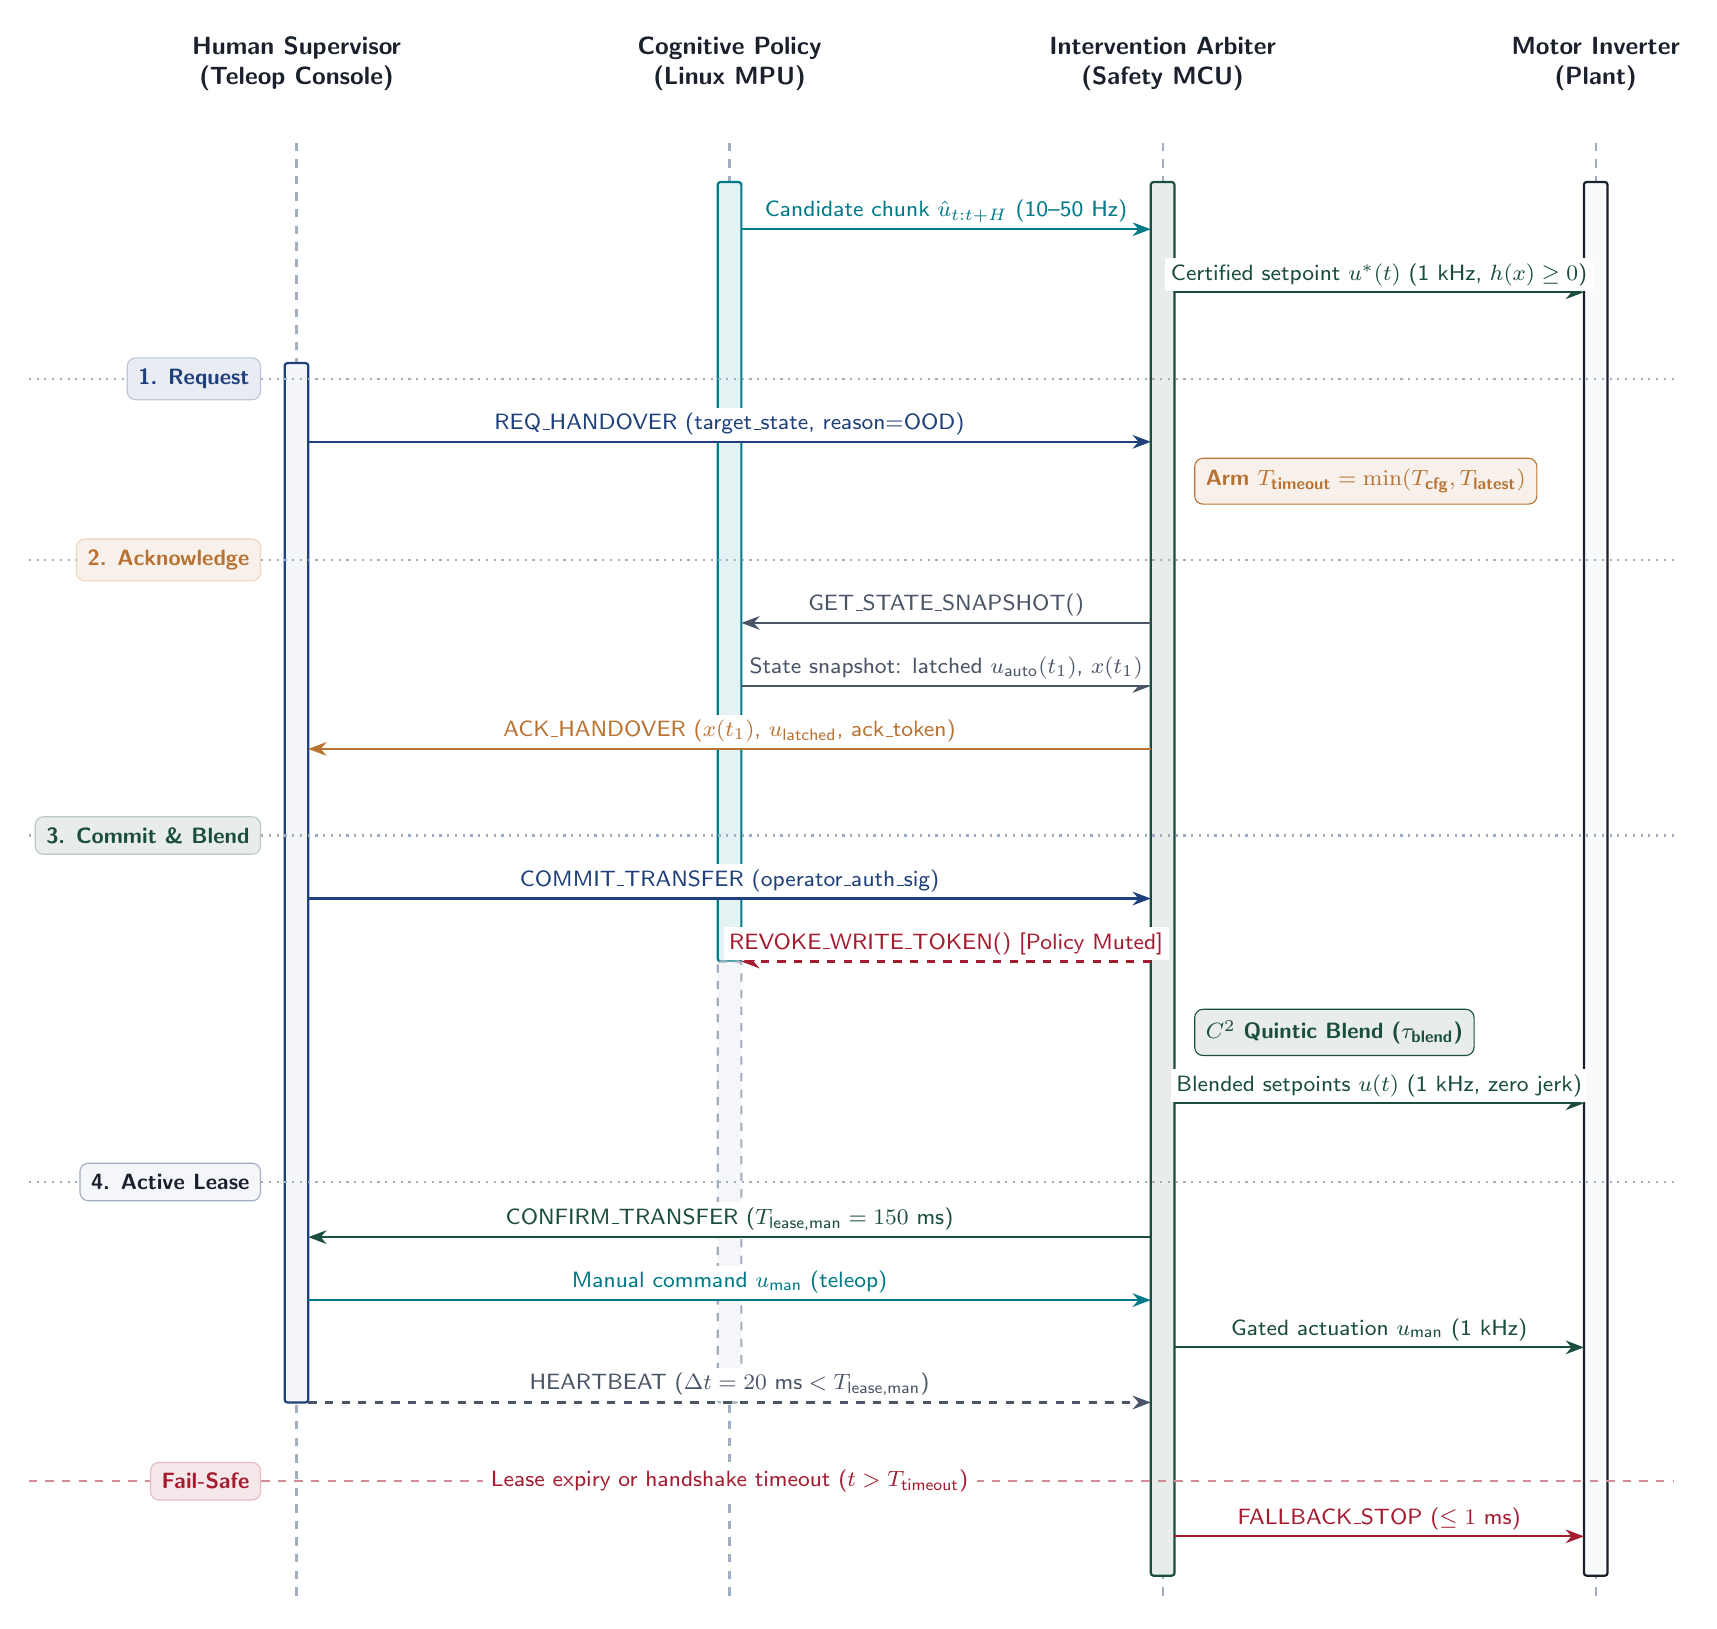
\begin{tikzpicture}[>=Stealth,
    header/.style={font=\sffamily\bfseries\small, text=ink, align=center},
    lifeline/.style={draw=paleink, dashed, thick},
    activation/.style={draw, rounded corners=1pt, thick},
    msg/.style={font=\sffamily\footnotesize, align=center, fill=white, inner sep=2pt},
    phasebox/.style={fill=shadecolor, draw=paleink, rounded corners=3pt, font=\sffamily\footnotesize\bfseries, inner sep=4pt},
    timeline/.style={draw=paleink, dotted, thick}
]

% Headers
\node[header] (hSup) at (0, 0) {Human Supervisor\\(Teleop Console)};
\node[header] (hPol) at (5.5, 0) {Cognitive Policy\\(Linux MPU)};
\node[header] (hArb) at (11, 0) {Intervention Arbiter\\(Safety MCU)};
\node[header] (hAct) at (16.5, 0) {Motor Inverter\\(Plant)};

% Lifelines
\draw[lifeline] (0,-1) -- (0,-19.5);
\draw[lifeline] (5.5,-1) -- (5.5,-19.5);
\draw[lifeline] (11,-1) -- (11,-19.5);
\draw[lifeline] (16.5,-1) -- (16.5,-19.5);

% Activations
\draw[activation, draw=ethdarkblue, fill=ethdarkblue!5] (-0.15, -3.8) rectangle (0.15, -17.0);
% Cognitive policy is active until write token revocation at -11.4
\draw[activation, draw=ethpetrol, fill=ethpetrol!10] (5.35, -1.5) rectangle (5.65, -11.4);
% Muted policy activation from -11.4 to -17.0
\draw[activation, draw=paleink, fill=shadecolor, dashed] (5.35, -11.4) rectangle (5.65, -17.0);
\draw[activation, draw=emeraldpine, fill=emeraldpine!10] (10.85, -1.5) rectangle (11.15, -19.2);
\draw[activation, draw=ink, fill=cardbg] (16.35, -1.5) rectangle (16.65, -19.2);

% Initial
\draw[->, draw=ethpetrol, thick] (5.65, -2.1) -- (10.85, -2.1) node[midway, above, msg, text=ethpetrol] {Candidate chunk $\hat{u}_{t:t+H}$ (10--50 Hz)};
\draw[->, draw=emeraldpine, thick] (11.15, -2.9) -- (16.35, -2.9) node[midway, above, msg, text=emeraldpine] {Certified setpoint $u^*(t)$ (1 kHz, $h(x) \ge 0$)};

% Phase 1
\draw[timeline] (-3.4, -4.0) -- (17.5, -4.0);
\node[phasebox, fill=ethdarkblue!10, draw=ethdarkblue!30, text=ethdarkblue, anchor=east] at (-0.45, -4.0) {1. Request};

\draw[->, draw=ethdarkblue, thick] (0.15, -4.8) -- (10.85, -4.8) node[midway, above, msg, text=ethdarkblue] {REQ\_HANDOVER (target\_state, reason=OOD)};

\node[phasebox, fill=ethbronze!10, draw=ethbronze, text=ethbronze, anchor=west] at (11.4, -5.3) {Arm $T_{\text{timeout}} = \min(T_{\text{cfg}}, T_{\text{latest}})$};

% Phase 2
\draw[timeline] (-3.4, -6.3) -- (17.5, -6.3);
\node[phasebox, fill=ethbronze!10, draw=ethbronze!30, text=ethbronze, anchor=east] at (-0.45, -6.3) {2. Acknowledge};

\draw[->, draw=softink, thick] (10.85, -7.1) -- (5.65, -7.1) node[midway, above, msg, text=softink] {GET\_STATE\_SNAPSHOT()};
\draw[->, draw=softink, thick] (5.65, -7.9) -- (10.85, -7.9) node[midway, above, msg, text=softink] {State snapshot: latched $u_{\text{auto}}(t_1)$, $x(t_1)$};
\draw[->, draw=ethbronze, thick] (10.85, -8.7) -- (0.15, -8.7) node[midway, above, msg, text=ethbronze] {ACK\_HANDOVER ($x(t_1)$, $u_{\text{latched}}$, ack\_token)};

% Phase 3
\draw[timeline] (-3.4, -9.8) -- (17.5, -9.8);
\node[phasebox, fill=emeraldpine!10, draw=emeraldpine!30, text=emeraldpine, anchor=east] at (-0.45, -9.8) {3. Commit \& Blend};

\draw[->, draw=ethdarkblue, thick] (0.15, -10.6) -- (10.85, -10.6) node[midway, above, msg, text=ethdarkblue] {COMMIT\_TRANSFER (operator\_auth\_sig)};
\draw[->, draw=harvardcrimson, thick, dashed] (10.85, -11.4) -- (5.65, -11.4) node[midway, above, msg, text=harvardcrimson] {REVOKE\_WRITE\_TOKEN() [Policy Muted]};

\node[phasebox, fill=emeraldpine!10, draw=emeraldpine, text=emeraldpine, anchor=west] at (11.4, -12.3) {$C^2$ Quintic Blend ($\tau_{\text{blend}}$)};

\draw[->, draw=emeraldpine, thick] (11.15, -13.2) -- (16.35, -13.2) node[midway, above, msg, text=emeraldpine] {Blended setpoints $u(t)$ (1 kHz, zero jerk)};

% Phase 4
\draw[timeline] (-3.4, -14.2) -- (17.5, -14.2);
\node[phasebox, fill=shadecolor, draw=paleink, text=ink, anchor=east] at (-0.45, -14.2) {4. Active Lease};

\draw[->, draw=emeraldpine, thick] (10.85, -14.9) -- (0.15, -14.9) node[midway, above, msg, text=emeraldpine] {CONFIRM\_TRANSFER ($T_{\text{lease,man}} = 150\text{ ms}$)};
\draw[->, draw=ethpetrol, thick] (0.15, -15.7) -- (10.85, -15.7) node[midway, above, msg, text=ethpetrol] {Manual command $u_{\text{man}}$ (teleop)};
\draw[->, draw=emeraldpine, thick] (11.15, -16.3) -- (16.35, -16.3) node[midway, above, msg, text=emeraldpine] {Gated actuation $u_{\text{man}}$ (1 kHz)};

\draw[->, draw=softink, thick, dashed] (0.15, -17.0) -- (10.85, -17.0) node[midway, above, msg, text=softink] {HEARTBEAT ($\Delta t = 20\text{ ms} < T_{\text{lease,man}}$)};

% Fail-Safe
\draw[timeline, draw=harvardcrimson!50, dashed] (-3.4, -18.0) -- (17.5, -18.0);
\node[phasebox, fill=harvardcrimson!10, draw=harvardcrimson!30, text=harvardcrimson, anchor=east] at (-0.45, -18.0) {Fail-Safe};
\node[msg, text=harvardcrimson, fill=white, inner sep=3pt] at (5.5, -18.0) {Lease expiry or handshake timeout ($t > T_{\text{timeout}}$)};

\draw[->, draw=harvardcrimson, thick] (11.15, -18.7) -- (16.35, -18.7) node[midway, above, msg, text=harvardcrimson] {FALLBACK\_STOP ($\le 1\text{ ms}$)};

\end{tikzpicture}
\end{document}
